\documentclass{article}
\usepackage[english]{babel}
\usepackage[letterpaper,top=2cm,bottom=2cm,left=3cm,right=3cm,marginparwidth=1.75cm]{geometry}

\usepackage{amsmath}
\usepackage{graphicx}
\usepackage{indentfirst}
\usepackage{amsfonts}
\usepackage[colorlinks=true, allcolors=blue]{hyperref}

\usepackage{upgreek}

% according devide the tag
\numberwithin{equation}{section}

\title{Model Predictive Control in Adaptive Cruise Control}
\author{Shuhao Bian}

\begin{document}
\maketitle

\begin{abstract}
    This paper proposes a novel approach to implementing Adaptive Cruise Control (ACC)
    using Model Predictive Control (MPC). MPC is a well-established technique for solving
    optimal control problems, and we demonstrate how it can be applied to the design of ACC
    systems. Specifically, we develop a linear model of the system and modify the MPC algorithm
    using a multiple shooting method and a technique for dynamically adjusting the MPC parameters
    during the optimization process. Our results demonstrate the effectiveness of this approach in
    achieving smooth and efficient vehicle control in a range of driving scenarios. Overall, this
    work offers a valuable contribution to the field of autonomous driving, providing a new
    perspective on the design of ACC systems.
\end{abstract}

\section{Problem Discreption}
% Adaptive Cruise Control (ACC) is a driver assistance system that uses radar, lidar, 
% or other sensors to detect the distance between your vehicle and the vehicle in front of you, 
% and automatically adjusts your vehicle's speed to maintain a safe following distance. 
% The system is designed to reduce the driver's workload, improve safety, 
% and increase comfort during long drives.

% The aim of ACC is to help drivers maintain a safe distance from the vehicle in front 
% of them, especially in heavy traffic or on long trips. ACC is also intended to reduce 
% driver fatigue and improve fuel efficiency by optimizing speed and acceleration. 
% Additionally, ACC can alert drivers to potential collisions and provide automatic 
% braking in emergency situations. Overall, ACC can make driving safer and more comfortable, 
% while reducing the risk of accidents and improving fuel efficiency.~\cite{1337334}

Adaptive Cruise Control (ACC) is an advanced driver assistance system designed
to automatically regulate a vehicle's speed in order to maintain a safe
following distance from the vehicle ahead. By utilizing a combination of
sensors, such as radar or LiDAR, and cameras, the ACC system continuously
monitors the relative velocity and distance between the two vehicles, as
illustrated in the accompanying figure. When the system detects that the
vehicle ahead is slowing down or if the following distance becomes too short,
it automatically adjusts the vehicle's speed by applying the brakes or reducing
throttle input. Conversely, when the traffic flow resumes or the distance
increases, the system will accelerate the vehicle back to its pre-set speed.
This not only enhances driving comfort and convenience but also contributes to
improved road safety and traffic flow efficiency.

\begin{figure}[h!]
    \centering
    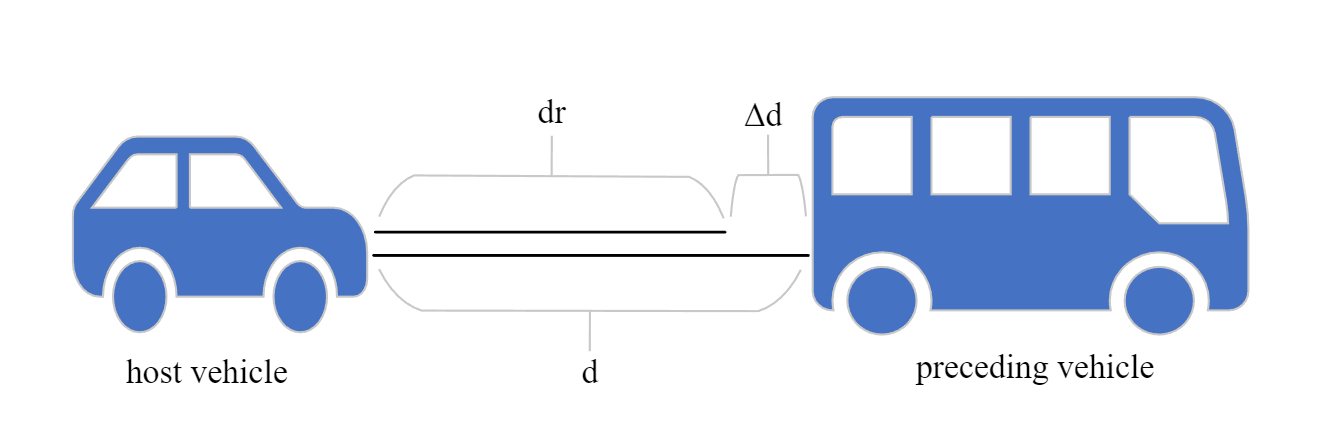
\includegraphics[width=0.5\textwidth]{host vehicle and preceding vehicle.png}
    \caption{Adaptive Cruise Control System}
    \label{fig:structure}
\end{figure}

Although Model Predictive Control (MPC)~\cite{rawlings2012postface} is a
popular method for solving the ACC problem, it still presents challenges due to
the computational load involved in solving large-scale optimization problems.
Therefore, this paper proposes a method to linearize the ACC system model and
use the powerful CasADi toolbox~\cite{Andersson2018} for solving the optimal
control problem.

\section{Formulation}

\subsection{ACC system}
% inter vhicle following error
In this paper, there are three parameters that can be measured as below by the
ACC system:
\begin{itemize}
    \item $\Delta d$: Inter-vehicle distance following error which is shown in Figure~\ref{fig:structure}, it represents the error between the
          desired inter-vehicle distance $d_r$ and actual inter-vehicle distance $d$. st. $\Delta d=d-d_r$.
          It's supposed to converge to zero if the ACC system works well.
    \item $\Delta v$: The speed following error, it represents the speed error between the
          host vehicle speed $v_h$ and target vehicle speed $v_r$. st. $\Delta v=v_h-v_r$.
          It's supposed to converge to zero.
    \item $\dot{v_h}$: the acceleration of the host vehicle. It's supposed to converge to
          be zero if target vehicle speed $v_r$ is constant. Because it's a simple linear model, we
          suppose the velocity of the target vehicle is constant.
\end{itemize}
\subsection{Vehicle Dynamics}
A vehicle dynamics model\cite{Takahama} will be used to describe the vehicle
dynamics and to build the MPC. The logitudinal dynamics of the host vehicle is
given by (\ref{eq:logitudinal_d}):

\begin{equation}
    \begin{aligned}
        m\dot{v_h}=F_f-r_{travel}\label{eq:logitudinal_d} \\
    \end{aligned}
\end{equation}

\noindent where $m$ is the mass of the host vehicle, $F_f$ is the total traction force of the host vehicle,
$r_{travel}$ is the rolling resistance of the host vehicle. The input/output relationship of
the vehicle dynamics model is given by the differential equation (\ref{eq:actuation_d}):

\begin{equation}
    \left\{\begin{array}{l}\label{eq:actuation_d}
        \dot{x}_{f}=f_{a c t}\left(x_{f}, u\right) \\
        a_{f}=h_{a c t}\left(x_{f}\right)
    \end{array}\right.
\end{equation}

\noindent where $x_f=\mathbb{R}^{n_{f}}$ is the state of the vehicle dynamics model, $u$ is the input of the
vehicle system~(\ref{eq:actuation_d}) which is often a control input calculated by embeded
micro cruise controller. $r_{travel}$ is travel resistance which can be calculated by the
following equation~(\ref{eq:travel_resistance}):

\begin{equation}
    r_{travel}=r_{air}v_h^2 + r_{roll}(v_h)+r_{accel}\dot{v_h}+r_{grad}(\theta)\label{eq:travel_resistance}
\end{equation}

\noindent where $r_{air}$ is the air resistance coefficient, $r_{roll}$ is the rolling resistance,
the $r_{accel}$ is the acceleration resistance coefficient, $r_{grad}$ is the gradient resistance,
$\theta$ is the slope angle.

\subsection{State-Space Model for ACC System}

To construct a plant model of the Adaptive Cruise Control (ACC) system, it is
necessary to consider both the desired inter-vehicle distance $d_r$ and the
minimum inter-vehicle distance $d_0$.

\begin{equation}
    d_r = T_{hw}v_h+d_0\label{eq:inter_vehicle_distance}
\end{equation}

\noindent where $T_{hw}$ is the headway time, $d_0$ is the minimum inter-vehicle distance.

In this paper, the state variables of the ACC system are as $x=[\Delta d,\Delta
    v,x_f^T]^T$, $x\in \mathbb{R}^{2+n_f}$, the state-space model is formulated as
(\ref{eq:state_space_model}):

\begin{equation}
    \left\{\begin{array}{l}\label{eq:state_space_model}
        \dot{x}=f_{a c t}\left(x, u\right) + Gv + Hw \\
        y=Cx+Jv
    \end{array}\right.
\end{equation}

\noindent where
$f_{a c t}(x,u)=\left[\begin{array}{c}
            \Delta v-T_{h w} x_{f}       \\
            -h_{a c t}\left(x_{f}\right) \\
            f_{a c t}\left(x_{f}, u\right)
        \end{array}\right], \quad G=\left[\begin{array}{c}
            T_{h w} / m \\
            1 / m       \\
            0
        \end{array}\right], \quad H=\left[\begin{array}{l}
            0 \\
            1 \\
            0
        \end{array}\right],C=\left[\begin{array}{lll}
            1 & 0 & 0 \\
            0 & 1 & 0 \\
            0 & 0 & 1
        \end{array}\right], \quad J=\left[\begin{array}{c}
            0 \\
            0 \\
            -1 / m
        \end{array}\right]$.

\noindent where $u \in \mathbb{R}$ is the input of the plant and
$y = [\Delta d, \Delta v, \dot{v_h}]^T \in \mathbb{R}^{3}$ is the output of the plant.

\section{Optimal-based Control Method}

\subsection{Controller Model Design}
In order to reduce the computational cost, the ACC system model is linearized
as (\ref{eq:linearized_model}):

\begin{equation}
    \left\{\begin{array}{l}\label{eq:linearized_model}
        \dot{a_f}=A_f(t)a_f+B_f(t)u \\
        a_f=C_fx_f
    \end{array}\right.
\end{equation}

\noindent where the acceleration of the linearized model is $a_f\in \mathbb{R}$, the input of the
linearized model is $u$, the output of the linearized model is $a_f$ and $A_f(t)$, $B_f(t)$, $C_f$ are
shown as (\ref{eq:linearized_m}):

\begin{equation}
    \begin{array}{l}\label{eq:linearized_m}
        A_{f}(t)=\left\{\begin{array}{ll}
                            -\frac{1}{T_{e n g}}, & \text { if } u(t) \geq a_{t h r_{-} o f f} \\
                            -\frac{1}{T_{b r k}}, & \text { if } u(t)<a_{t h r_{-} o f f}
                        \end{array}\right.                                  \\
        B_{f}(t)=\left\{\begin{array}{ll}
                            \frac{K_{e n g}(t)}{T_{e n g}}, & \text { if } u(t) \geq a_{t h r_{-} o f f} \\
                            \frac{K_{b r k}(t)}{T_{b r k}}, & \text { if } u(t)<a_{t h r_{-} o f f}
                        \end{array}\right. \\
        C_{f}=1 .
    \end{array}
\end{equation}

\noindent where $T_{e n g}$ is the constant of acceleration of acceleration engine,
$T_{b r k}$ is time constant of deceleration using brake, $a_{t h r_{-} o f f}$ is the threshold
of acceleration, $K_{e n g}(t)$ and $K_{b r k}(t)$ are the gain of acceleration engine and brake
respectively.

In the system (\ref{eq:linearized_model}), the dynamics of the vehicle is
simplified as a first-order delay system. The system has two modes:a
acceleration mode and a deceleration mode.

So the prediction model (\ref{eq:state_space_model}) can be simplified as
(\ref{eq:prediction_m}).

\begin{equation}
    \left\{\begin{array}{l}\label{eq:prediction_m}
        \dot{x}=A(t)x+B(t)u+Gv+Hw \\
        y=Cx+Jv
    \end{array}\right.
\end{equation}

\noindent where $x \in \mathbb{R}^3$ and $A(t)=\left[\begin{array}{ccc}
            0 & 1 & -T_{h w} \\
            0 & 0 & -1       \\
            0 & 0 & A_{f}(t)
        \end{array}\right], \quad B(t)=\left[\begin{array}{c}
            0 \\
            0 \\
            B_{f}(t)
        \end{array}\right]$.

We use the prediction model based on \ref{eq:prediction_m} and assume that the
disturbance $v$ and $w$ are unmeasurable.
\subsection{Optimization Problem of MPC}

MPC is considered suboptimal compared to optimal control strategies, as it
provides an approximate solution to the optimal control problem. This
suboptimality arises from factors such as the use of a finite prediction
horizon, which may not fully account for the consequences of control actions;
inaccuracies in the system's mathematical model, which can lead to suboptimal
predictions and control decisions; discretization and approximations required
for representing constraints or nonlinear dynamics; and computational
constraints in real-time applications, necessitating the use of simplified
optimization algorithms or problem formulations.

While comparing MPC's performance to that of an optimal controller can be
challenging, especially for complex or high-dimensional systems, the
qualitative argument for its suboptimal nature remains valid. Despite being
suboptimal, MPC continues to be widely adopted in practice due to its practical
advantages and overall satisfactory performance.

Because the model of the MPC system in this paper is linear, so it can be
considered a convex problem\cite{LIMON20082382}. Convex optimization problems
have a unique global minimum and can usually be solved efficiently using linear
programming (for linear objective functions) or quadratic programming (for
quadratic objective functions) techniques.

% In this paper, the MPC controller is designed to minimize the following

\subsection{MPC Controller Design}

The relationship between the prediction horizon and the controller performance
is crucial, as it impacts the controller's ability to respond to changes in the
system and its overall effectiveness.
\begin{itemize}
    \item Short prediction horizon: A short prediction horizon may lead to faster
          computation times since the optimization problem has fewer variables and
          constraints. However, it may result in suboptimal control performance, as the
          controller has limited foresight and may not adequately account for future
          disturbances, constraints, or desired setpoints. This can lead to overly
          aggressive or reactive control actions.

    \item Long prediction horizon: A longer prediction horizon allows the controller to
          better anticipate future events and make more informed control decisions. This
          can lead to improved performance, smoother control actions, and a better
          ability to handle disturbances and constraints. However, longer prediction
          horizons come at the cost of increased computational complexity, which may
          result in slower optimization and potentially reduced control update rates.
          Moreover, the quality of the model and the predictability of the system may
          degrade over longer horizons, leading to diminishing returns on controller
          performance.
\end{itemize}

According to the law above, we prefer to have a shorter horizon when the
distance is long because we need more aggressive control actions to achieve the
desired distance. This is also a trade-off between the computational cost and
the performance of the controller.

When the distance is short, we prefer to have a longer horizon because we need
to consider more future events and make more informed control decisions. And we
need to consider the confort of the driver.

So we designed the strategy of the MPC controller as the figure
\ref{fig:mpc_design}.
\begin{figure}[h!]
    \centering
    \includegraphics[width=0.5\textwidth]{ACC MPC/mpc design.png}
    \caption{The structure of the MPC controller}
    \label{fig:mpc_design}
\end{figure}

Because the model dynamics $\dot{x}=f(x,u)$ are unstable in the prediction
horizon, we need to update the state $x$ in each time step. So we use the
multiple shooting method to solve the optimization problem.

Multiple shooting is a numerical optimization technique used to solve optimal
control problems, including those arising in Model Predictive Control (MPC).
The main idea behind multiple shooting is to divide the prediction horizon into
several smaller intervals or subproblems, and then solve these subproblems
simultaneously while ensuring continuity of the states and inputs across the
intervals. In this way, the optimization problem is decomposed into a sequence
of smaller problems, each of which can be solved efficiently using standard
optimization techniques.

In multiple shooting method, the model dynamics are discretized on a uniform
time grid $t_0, ..., t_N$ by numerical integration over the time intervals
$[t_i, t_{i+1}]$. The control input $U$ is assumed to be constant over each
interval, and the state $X$ is updated at the end of each interval. The
inequality constraints are enforced at the end of each interval.

\section{Numerical Simulation and Results}
Numerical simulations were performed to evaluate the performance of the
proposed MPC controller. The control performance was compared with the
performance of a method using single shooting method and a method using common
MPC controller.

In the simulation, the controller's sampling time is 0.1s, the control input
and its change rate ahve the lower and upper limit $u \in [-2.5,1.5]$ and
$\Delta u \in [-1.5,1.5]$, respectively. Table \ref{tab:parameters} shows the
parameters of the ACC system.

% insert a table
\begin{table}[h!]
    \centering
    \caption{The parameters of the ACC system}
    \begin{tabular}{|c|c|}
        \hline
        Parameter & Value \\
        \hline
        $T_{eng}$ & 0.46  \\
        \hline
        $T_{eng}$ & 0.732 \\
        \hline
        $h_w$     & 1.6
    \end{tabular}
    \label{tab:parameters}
\end{table}

Python CasADi were used in the simulation. The optimization problem is solved
by IPOPT solver in CasADi.

In the figure \ref{fig:adaptive_mpc} and figure \ref{fig:common_mpc}, the
common MPC is more aggressive than the proposed MPC when the car are very close
to the desired distance which may cause the driver uncomfortable.

\begin{figure}[h!]
    \centering
    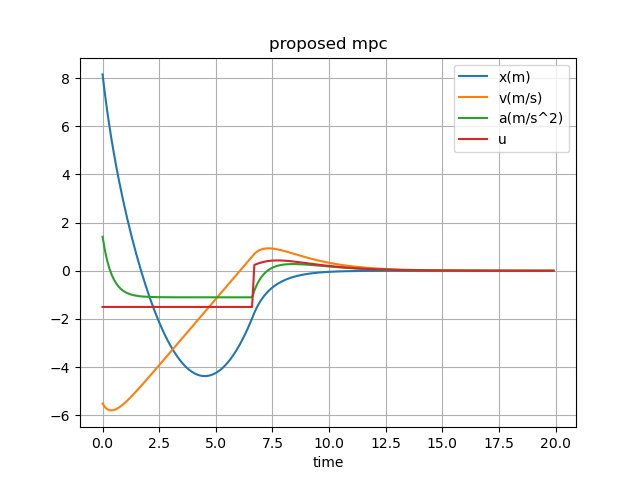
\includegraphics[width=0.5\textwidth]{ACC MPC/proposed mpc.png}
    \caption{the performance of proposed MPC}
    \label{fig:adaptive_mpc}
\end{figure}

\begin{figure}[h!]
    \centering
    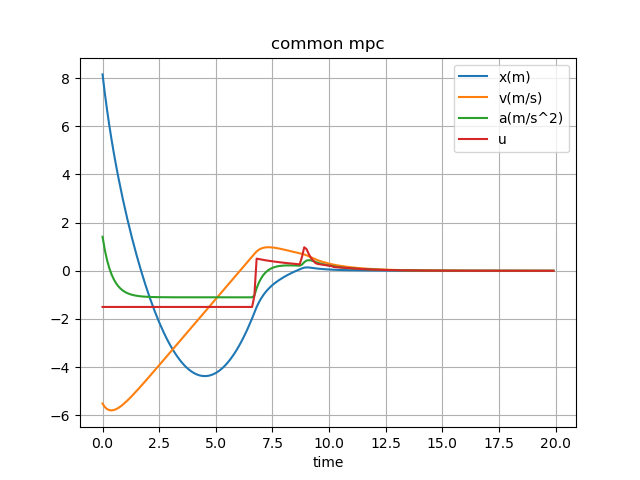
\includegraphics[width=0.5\textwidth]{ACC MPC/common mpc.png}
    \caption{the performance of common MPC}
    \label{fig:common_mpc}
\end{figure}

In the figure \ref{fig:proposed_mpc_with_dis} and figure
\ref{fig:common_mpc_with_dis}, the common MPC is more sensitive to the
disturbance than the proposed MPC and becomes unstable when the car is closed
to the desired distance. The proposed MPC can still keep the car close to the
desired distance when the disturbance is large.

\begin{figure}[h!]
    \centering
    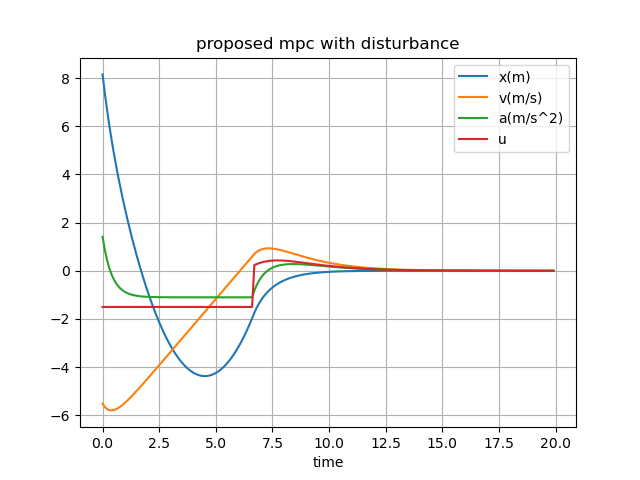
\includegraphics[width=0.5\textwidth]{ACC MPC/proposed mpc with disturbance.png}
    \caption{the performance of proposed MPC with disturbance}
    \label{fig:proposed_mpc_with_dis}
\end{figure}

\begin{figure}[h!]
    \centering
    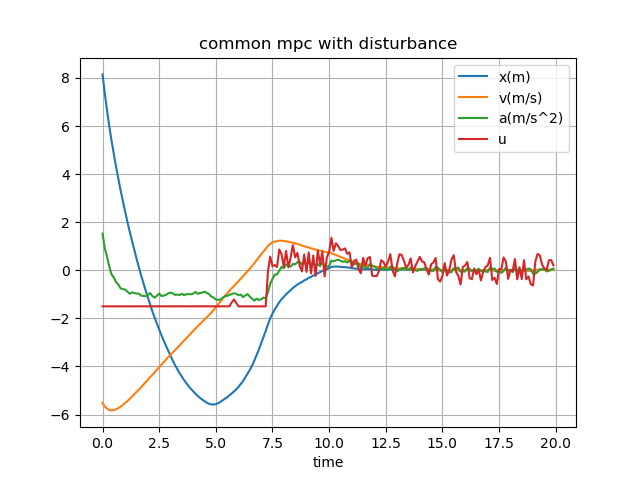
\includegraphics[width=0.5\textwidth]{ACC MPC/common mpc with disturbance.png}
    \caption{the performance of common MPC with disturbance}
    \label{fig:common_mpc_with_dis}
\end{figure}

As we can see from the figure \ref{fig:calculate_time}, the time consumption of
the proposed MPC with a multiple shooting approach is much less than that of
the common MPC with a single shooting approach.

\begin{figure}[h!]
    \centering
    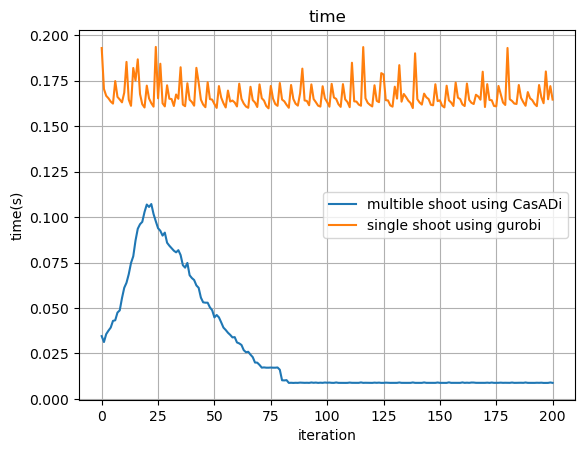
\includegraphics[width=0.5\textwidth]{ACC MPC/output.png}
    \caption{calculation time}
    \label{fig:calculate_time}
\end{figure}

\section{Conclusion}

In this paper, we proposed a MPC controller for ACC system. The simulation
results show that the proposed controller can achieve the desired performance.

What's more, we can adjusts the prediction horizon and control horizon of the
MPC controller according to the distance between the vehicle and the front
vehicle. By choosing multiple shooting method, the calculation time of the MPC
controller is reduced.

\bibliographystyle{unsrt}
\bibliography{citation}

\end{document}